\documentclass[a4paper,11pt]{article}

% Packages for page layout
\usepackage[utf8]{inputenc}
\usepackage{fancyhdr}
\usepackage{lastpage}

% Minted for syntax highlighting
\usepackage{minted}
\usemintedstyle{tango}

% Custom paragraph indentation
\setlength{\parindent}{0em}
\setlength{\parskip}{1em}
 
% Headers/footers styling
\pagestyle{fancy}
\fancyhf{}
\renewcommand{\headrulewidth}{0pt}

% Footer
\lfoot{ID1019}
\cfoot{KTH}
\rfoot{\thepage \hspace{1pt} / \pageref{LastPage}}

% Finite state machines
\usepackage{tikz}
\usetikzlibrary{automata,arrows,topaths}


% SECTIONS
%
% * Introduction
% * The splay tree
% * The implementation
% * Why this exercise
% * Summary


\begin{document}

% ================================================== %
% == Title == %
% ================================================== %

\title{
    \textbf{Splay Trees}\\
    \large{Programming II - Elixir Version}
}
\author{Johan Montelius}
\date{Spring Term 2018}
\maketitle
\thispagestyle{fancy}


% ================================================== %
% == Introduction == %
% ================================================== %

\section*{Introduction}

A splay tree is an ordered binary tree with the advantage that the
last key we looked for is found in the root of the tree. We will 
rearrange the tree in every access, moving the key to the top and
trying to keep the rest of the tree balanced.

The amortized cost of operations (search, insert, delete) are all
$O(lg(n))$. There are worst case scenarios, since there is no
guarantees that the tree is balanced, but we accept this since the data
structure has its advantages. Frequently used keys will be found
higher up in the tree so it is very good to use in an application
where we expect temporal locality i.e. if you have used one key it is
very likely that you will use this key again with in a short period of time.

In this assignment you're going to learn how to implement a quite
tricky algorithm using pattern matching. You should look up some
tutorial on splay trees so that you have a basic understanding of the
algorithm but we will explain the algorithm as we go along. We will
first look at the general idea of these operations using a graphical
representation before going in to how to implement it in Elixir. 


% ================================================== %
% == The splay tree == %
% ================================================== %

\section{The splay tree}

In this implementation we will create a splay tree that keeps
key-value pairs. The key-values will reside in all of the nodes
besides the leafs which are empty branches. The tree is ordered with
smaller values in left branches.

Doing search in this tree is of course trivial but we will do a search
where we also change the structure of the tree. This is the key
operation in all splay tree operations; updating, lookup and insertion
are essentially the same algorithms since they all perform the same
transformation.


In this description we will first look at the operation to update or
insert a value given a key. If the key is present we will update the
value, if not we will add the key-value pair. Once we understand how
this is done it will be easy to implement the other operations. 

The splay operation is slightly different depending on if we are in
the root of the tree or doing a recursive operation further down in
the tree. Before explaining the general rules let's look at the rules
for the root.

\subsection{Splay of the root}
Assume that we want to update a value for a key in a tree. We will
have two very easy special cases when the tree is empty or if the key
is found in the root of the tree. In these cases we simply return a
tree with one node or update the existing root with the new
value. 

The splay operation comes in when we find the key in one of the
branches. We should then rearrange the tree in a way that moves the key 
to root of the tree. The operation is quite straight forward as seen
in the graph shown in figure~\ref{fig:root}. 

Note that the lefter-most sub-tree, {\em A}, of course contains keys
that are less than the key ({\em K}) that we're looking for and it is safe to
have it as the left branch of the new tree. The sub-tree {\em B}
contains keys that are greater than the key we are looking for but
smaller than the key of the root ({\em R}) . Its position in the transformed tree
is therefore sound. The same thing goes for the sub-tree {\em C} that
must contain keys that are greater than the key of the root.

There is s corresponding splay operations when we find the key in the
left branch. Write it down using the same naming scheme as in in
figure~\ref{fig:root}. This will make the implementation step easier.

\begin{figure}
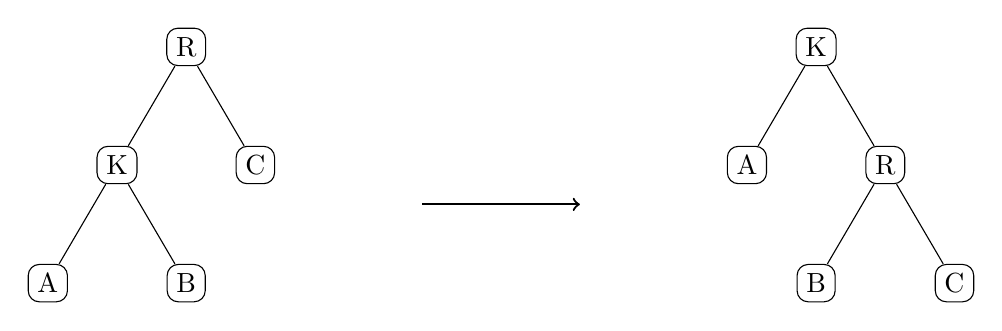
\begin{tikzpicture}[sibling distance=5em,
  every node/.style = {shape=rectangle, rounded corners, draw, align=center}]]

  \node at (2,4) {R} 
    child { node {K} 
      child { node {A} }
      child { node {B} } }
    child { node {C}};

  \draw[thick, ->] (5,2) -- (7,2);

  \node at (10,4) {K} 
    child { node {A}}
    child { node {R} 
        child { node {B} }
        child { node {C} }};

\end{tikzpicture}
\caption{Zig: splay operation of the root when the key (K) is found in left branch. \label{fig:root}}
\end{figure}

\pagebreak

\subsection{Splay further down the tree}
In general the splay operation on a tree will result in a tree where
the key that we're updating becomes the root of the tree. The
operation looks very similar to the operation that we have seen for
the root of the tree, the only difference is that we now look further
down the tree before determining what to do. We first describe the
general rules before describing the special cases.

We have four cases and we could call them
left-left, left-right etc but for historic reasons we call them:
zig-zig, zig-zag, zag-zig and zag-zag. We only show the two first
since the two other are mirror images of the two first.

When describing these rules we use the naming 'K' for the node
where the key is found, 'P' for the parent node and 'G'
for the grandparent. Sub-trees that are moved around are called
'A', 'B' etc and we write them in an order so that we
know that all keys in for example sub-tree 'A' are smaller than
keys in sub-tree 'B'. We will later use these names for
variables in our implementation so let's try to be consistent.

\subsubsection*{Zig-zig}
The zig-zig rule is used if we find the key in the lefter-left node. In
figure~\ref{fig:zigzig} we see how we move the node holding the key we're
looking for ({\em K}) to the root and rearrange the parent
({\em P}), and grandparent ({\em G}), to form the new tree. Note
the order of the sub-trees {\em A}, {\em B}, {\em C} and
{\em D}.  Make sure that you understand why it is safe to do the
transformation of the tree and why the tree is still ordered.
 
\begin{figure}
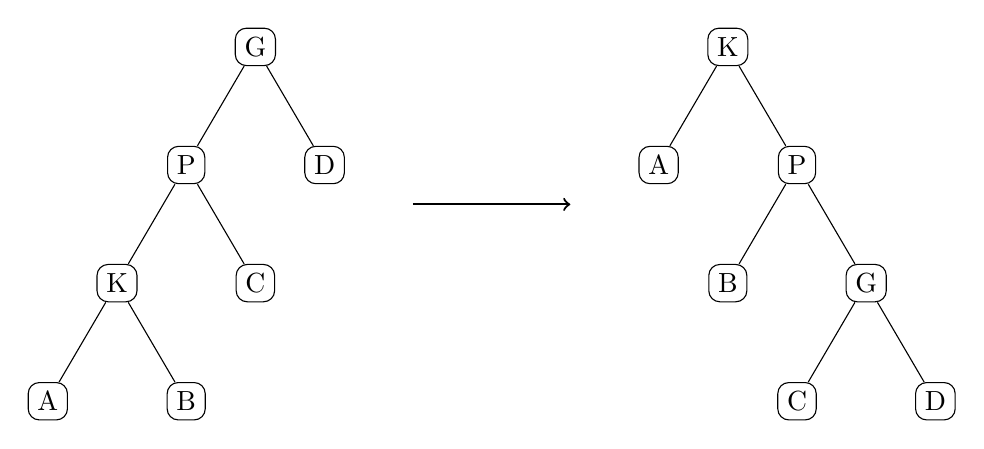
\begin{tikzpicture}[sibling distance=5em,
  every node/.style = {shape=rectangle, rounded corners, draw, align=center}]]

  \node at (2,4) {G} 
    child { node {P} 
      child { node {K} 
         child { node {A} }
         child { node {B} } }
      child { node {C} } }
    child { node {D}};

  \draw[thick, ->] (4,2) -- (6,2);

  \node at (8,4) {K} 
    child { node {A}}
    child { node {P} 
        child { node {B} }
        child { node {G} 
          child { node {C}}
          child { node {D}}}};

\end{tikzpicture}
\caption{Zig-Zig: splay operation when key is found in left-left branch. \label{fig:zigzig}}
\end{figure}


\subsubsection*{Zig-zag}
The second rule covers the case where we find the key in the
left-right node. The transformation is a little different but the aim
is the same; move the key to the root and rearrange the sub-trees to
keep the tree ordered. In figure~\ref{fig:zigzag} we see how the
transformation is done.

\begin{figure}
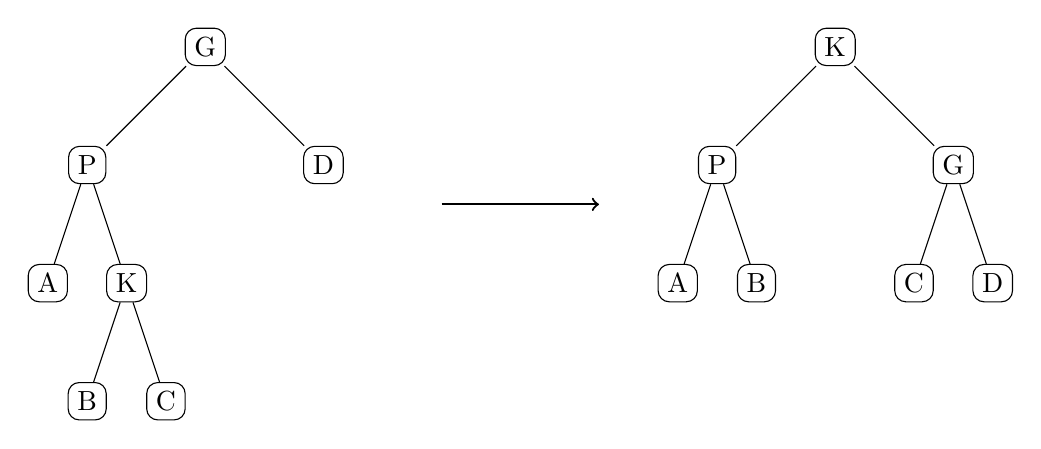
\begin{tikzpicture}[every node/.style = {shape=rectangle, rounded corners, draw, align=center},
level 1/.style={sibling distance=30mm},level 2/.style={sibling distance=10mm}]]

  \node at (2,4) {G} 
    child { node {P} 
      child { node {A}}
      child { node {K} 
         child { node {B} }
         child { node {C} } }}
    child { node {D}};

  \draw[thick, ->] (5,2) -- (7,2);

  \node at (10,4) {K} 
    child { node {P} 
        child { node {A} }
        child { node {B} }}
    child { node {G}
          child { node {C}}
          child { node {D}}};
\end{tikzpicture}
\caption{Zig-Zag: splay operation when the key (K) is found in left-right branch. \label{fig:zigzag}}
\end{figure}

\subsection{Zag-zig and zag-zag}

The two described rules of course have their mirror rules when the key
is found in either the right-right or right-left node.  The idea is
the same, move the found key to the root and the parent node one level
down. The grandparent node becomes the child of either the parent node
or the key node.

You're strongly advised to draw the graphs that describes these
zag-zig and zag-zag rules. Keep the naming of nodes: {\em G} for
grandparent, {\em P} for parent and {\em K} for the node where we find
the key. Sub-trees are called: {\em A}, {\em B } etc and are named in
order.

These are the complicated rules, what we have left are the very
simple rules for some base cases.

\subsection{Zig or zag or nil}
We have several base cases that cover the situations where the tree is
not very deep or when we find the key that we're looking for in one of
the two first levels. In the same way as for the root we could have an
empty tree or a tree where the key is in the root; these cases are
trivial. If the key is found in the root of either sub-tree we do a
transformation that is exactly the same transformation that we would
do for the root.

If the sub-tree where the key should be found is empty we do the same
operation as we would do if we found the key in the root of the
sub-tree. An example of what this looks like is seen in
figure~\ref{fig:nil}.

The rule is equivalent to the zig rule that we used in the root of the
tree. It of course has its corresponding zag versions where the key
should go into the right branch.

\begin{figure}
\begin{tikzpicture}[sibling distance=5em,
  every node/.style = {shape=rectangle, rounded corners, draw, align=center}]]

  \node at (2,4) {G} 
    child { node {} }
    child { node {C}};

  \draw[thick, ->] (5,2) -- (7,2);

  \node at (10,4) {K} 
    child { node {}}
    child { node {G} 
        child { node {} }
        child { node {C} }};

\end{tikzpicture}
\caption{Zig: splay operation when key should go into left branch. \label{fig:nil}}
\end{figure}

\pagebreak


% ================================================== %
% == The implementation == %
% ================================================== %

\section{The implementation}

We will implement a function {\tt update/3} that takes a splay tree, a
key and a value and returns a transformed splay tree where the key has
been updated or inserted if it was not present. In both cases the key
value pair is of course found in the root of the transformed tree.

A tree is represented by:
\begin{itemize}
  \item {\tt nil}:  the empty tree
  \item {\tt \{:node, key, value, left, right\}}:  a node with a key, value and a left and right branch
\end{itemize}

In the implementation we will use the same naming of nodes as in the
graphical representations. We will augment names with {\tt k} or {\tt
  v} depending on if we refer to the key or value. A key value pair
will for example be named {\tt rk} and {\tt rv} if it's the root
node. Nodes that are only moved around will be called {\tt a}, {\tt b}
etc.  The idea is that we should keep the implementation as close to
the graphical description as possible.

\subsection{Update of the root}
Let's start with the base cases for updating the root. We either have
a empty tree or a node where we are lucky enough to find the key in
the root. Below is the skeleton code that you should use, fill in the
blanks.

\begin{minted}{elixir}
def update(nil, key, value) do
  {:node, ..., ..., ..., ...}
end

def update({:node, key, _, a, b}, key, value) do
  {:node, ..., ..., ..., ...}
end
\end{minted}

The two general cases, {\em Zig} and  {\em Zag} are where we will do a
call to  a general {\em  splay} operation. The function  {\tt splay/2}
takes a  tree and a key  and will return  a tuple {\tt \{:splay,  kv, a,
  b\}} where {\tt kv}  is the value of the key ({\tt :na}  if the key is
not found) and {\tt a} and {\tt  b} the left and right sub-trees. When
we do an update of a value  we're not interested in the found value of
the key but we will use this in the coming operations.

If we know that {\tt splay/2} works for all trees then we can use it
to implement the zig and zag rules of the root.

\begin{minted}{elixir}
def update({:node, rk, rv, zig, c}, key, value) when key < rk do
  # The general rule where we will do the Zig transformation.
  {:splay, _, a, b} = splay(zig, key)
  {:node, ..., ..., ..., {:node, ..., ..., ..., ...}}
end

def update({:node, rk, rv, a, zag}, key, value) when key >= rk do
  # The general rule where we will do the Zag transformation.
  {:splay, _, b, c} = splay(zag, key)
  {:node, ..., ..., {:node, ..., ..., ..., ...}, ...}
end
\end{minted}

When you fill in the blank spots in the code, use variable names that
found in the graphical representations of the rules. This will help
you to verify that you're actually doing the right thing. If we now
only can implement the {\tt splay/2} function we are done.

\subsection{Splay of the tree}
As for the root we have two base cases when the tree is empty and when the key
is found in the root. These should be quite easy to write down.

\begin{minted}{elixir}
defp splay(nil, _) do
  {:splay, :na, ..., ...}
end

defp splay({:node, key, value, a, b}, key) do
  {:splay, ..., ..., ...}
end
\end{minted}

The general zig-zag rules only work if we have three levels to work
with. We therefore have two more special cases where the left or right
sub-tree is empty. We should still return a splay-tuple and therefore
need to construct two sub-trees. Make sure that you get this right,
what should go into the empty spaces.

\pagebreak

\begin{minted}{elixir}
defp splay({:node, rk, rv, nil, b}, key) when key < rk do
  # Should go left, but the left branch empty.
  {:splay, :na, ..., {:node, rk, rv, ..., ...}}
end
defp splay({:node, rk, rv, a, nil}, key) when key >= rk do
  # Should go right, but the right branch empty.
  {:splay, :na, {:node, rk, rv, ..., ...}, ...}
end
\end{minted}

One more special case is when the key is actually found as the root in
the left or right sub-tree. Very similar to the case above but now we
actually have a found a value.

\begin{minted}{elixir}
defp splay({:node, rk, rv, {:node, key, value, a, b}, c}, key) do
  # Found to the left.
  {:splay, ..., ..., {:node, ..., ..., ..., ...}}
end

defp splay({:node, rk, rv, a, {:node, key, value, b, c}}, key) do
  # Found to the right.
  {:splay, ..., {:node, ..., ..., ..., ...}, ...}
end
\end{minted}

When this is done we are ready for the general zig-zag rules. We here
list the complete coding of the zig-zig rule and you should complete
the remaining rules. The zig-zig rule applies the splay operation on
the left-left sub-tree and obtains the sub-trees {\tt a} and {\tt b}
that can then be used to rearrange the tree. Note that the splay
operation also provides the found value, {\tt kv}, and this value is
returned in the splay tuple.

\begin{minted}{elixir}
defp splay({:node, gk, gv, {:node, pk, pv, zig_zig, c}, d}, key) 
    when key < gk and key < pk do
  # Going down left-left, this is the so called zig-zig case. 
  {:splay, value, a, b} = splay(zig_zig, key)
  {:splay, value, a, {:node, pk, pv, b, {:node, gk, gv, c, d}}}
end
\end{minted}

The zig-zag rule is similar but now we have walked down the left-right
branch. Look at the graphical representation of the rule in
figure~\ref{fig:zigzag}. Fill in the blanks, which sub-trees should go
where?

\begin{minted}{elixir}
defp splay({:node, gk, gv, {:node, pk, pv, a, zig_zag}, d}, key)
    when key < gk and key >= pk do
  # Going down left-right, this is the so called zig-zag case. 
  ... = splay(zig_zag, key)
  {:splay, value, {:node, pk, pv, a, b}, {:node, gk, gv, ..., ...}}
end
\end{minted}

The remaining two rules are the mirror images of the first two
rules. If you have not done so yet you should draw the images of the
rules using the same naming strategy. There should be a one-to-one
mapping from drawn rules to clauses in the code. When your done you
have implemented the update function for splay trees.

\begin{minted}{elixir}
defp splay({:node, gk, gv, a, {:node, pk, pv, zag_zig, d}}, key)
    when key >= gk and ... do
  ...
  {:splay, value, {:node, gk, gv, a, b}, {:node, pk, pv, c, d}}
end

defp splay({:node, gk, gv, a, {:node, pk, pv, b, zag_zag}}, key)
    when ... do
  ...
  {:splay, value, {:node, pk, pv, {:node, gk, gv, a, b}, c}, d}
end
\end{minted}

This is it, you have implemented the update function of splay
trees. Write some small test examples that updates a tree, try this:

\begin{minted}{elixir}
def test() do
  insert = [{3, :c}, {5, :e}, {2, :b}, {1, :a}, {7, :g}, {4, :d} {5, :e}]
  empty = nil
  List.foldl(insert, empty, fn({k, v}, t) -> update(t, k, v) end)
end
\end{minted}


% ================================================== %
% == Why this exercise == %
% ================================================== %

\section{Why this exercise}

It's of course fun to implement an algorithm that you might have hear
off but not fully understood. The aim of this exercise is however not
the algorithm per see but how pattern matching and recursion can be
used to implement a fairly complicated algorithm.

I hope that you see how the graphical descriptions maps to patterns
and how easy it is to build the desired transformation. If you would
have implemented this algorithm from scratch, you would probably have
to do some thinking and experimenting before coming up with the
solution that we have now. Looking at the solution it looks obvious
but it takes some time to understand how to get the recursion right.

\subsection{A mutable solution}
The Elixir implementation that we have now does not not look like the
solution you would write in Java or C++. In Elixir, as almost all
functional programming languages, data structures are immutable and we
construct a new tree in each operation. In a language where you can
change data structures your would most likely change the structure of
the given tree.

If you implement the update procedure and change the structure of the
tree, you will most likely work with a linked tree where all nodes
know their immediate parent. The algorithm would then first traverse
down the tree to find the node with the given key, or construct one in
a leaf if it is not present, and then {\em splay} this node towards
the root using the parent pointers. 

You can probably work out what the algorithm looks like: if my parent
has a parent and I'm the left child of my parent and my parent is the
left child of its parent, then\ldots

\begin{minted}{cpp}
void splay( node *x ) {
  while( x->parent ) {
    if( !x->parent->parent ) {
      if( x->parent->left == x ) right_rotate( x->parent );
      else left_rotate( x->parent );
    } else if( x->parent->left == x && 
                x->parent->parent->left == x->parent ) {
      right_rotate( x->parent->parent );
      right_rotate( x->parent );
    } else if( x->parent->right == x && 
                x->parent->parent->right == x->parent ) {
      left_rotate( x->parent->parent );
      left_rotate( x->parent );
    } else if( x->parent->left == x && 
                x->parent->parent->right == x->parent ) {
      right_rotate( x->parent );
      left_rotate( x->parent );
    } else {
      left_rotate( x->parent );
      right_rotate( x->parent );
    }
  }
}
\end{minted}

The actual rotation operations are of course pointer manipulations
where the left, right and parents pointers are set to form the new
structure of the tree. Updating the data structure in place is of
course more efficient than building a new structure in each
transformations. Immutable data structures do however have their
advantage when it comes to robustness and possibility to run things in
parallel. What we look at now is however how expressive the different
approaches are when coding a complex algorithm.

\begin{minted}{cpp}
void right_rotate( node *x ) {
  node *y = x->left;
  if(y) {
    x->left = y->right;
    if( y->right ) y->right->parent = x;
    y->parent = x->parent;
  }
  if( !x->parent ) root = y;
  else if( x == x->parent->left ) x->parent->left = y;
  else x->parent->right = y;
  if(y) y->right = x;
  x->parent = y;
}
\end{minted}

\subsection{Structs and named fields}
Since we are looking at how easy it is to express an algorithm we can
take the opportunity to rewrite the program using Elixir structs. The
structs functionality will give us the ability to use named fields
instead of explicitly writing down a whole tuple in a pattern.

Assume that we have a struct definition for a node with the fields:
{\tt key}, {\tt value}, {\tt left} and {\tt right}. We could then
rewrite {\tt update/3} in the following way (we here also combine the
three alternatives in one clause).

\begin{minted}{elixir}
defstruct key: nil, value: nil, left: nil, right: nil

def update(nil, key, value) do
  %Node{key: key, value: value, left: nil, right: nil}
end

def update(%Node{} = node, key, value) do
  cond do
    key == node.key ->
      %Node{
        key: key,
        value: value,
        left: node.left,
        right: node.right
      }

    key < node.key ->
      {:splay, _, a, b} = splay(node.left, key)
      %Node{
        key: key,
        value: value,
        left: a,
        right: {:node, node.key, node.value, b, node.right}
      }

    true ->
      {:splay, _, b, c} = splay(node.right, key)
      %Node{
        key: key,
        value: value,
        left: {:node, node.key, node.value, node.left, b},
        right: c
      }
  end
end
\end{minted}

Using the structs we do not have to memorize the order of the
elements in the node structure. It makes it easier to update the code,
for example if we find that we need another element in each
node. Using explicit patterns is often the easier way of handling
things while the use of more complex data structures almost requires
that you use the struct functionality.


% ================================================== %
% == Summary == %
% ================================================== %

\section{Summary}

Pattern matching is a powerful technique to describe the rules of a
transformation. Together with recursion even a complex algorithm
becomes quite easy to implement. 

\end{document}
